\documentclass[12pt, oneside, notitlepage]{book}
% pls don't just add packages to solve problems. Check that it is not doable with existing packages, or ask if in doubt. To many packages slows down compilation time by alot!

\usepackage{titlesec}
\usepackage[acronym, toc,section=section]{glossaries} % Glossary support by using \gls{glossarykey.
\usepackage[hidelinks]{hyperref}  % Extensive support for hypertext in LATEX
\usepackage{graphicx} % allows usage of \includegraphics[options]{name} to include figures and similar.
\usepackage[style=ieee]{biblatex} % Bibliography.
%\usepackage[T1]{fontenc} % Changes font encoding to allow for newer fonts.
%\usepackage[english]{babel} % Language Support.
%\usepackage{caption} % Customising captions in floating environments
\usepackage[top=1in, bottom=1in, left=1in, right=1in]{geometry} % Change Margins, Padding etc.
\usepackage{float} % Improved interface for floating objects
%\usepackage[dvipsnames]{xcolor} % Easy way to set color for e.g. text: \textcolor{color}{text}
%\usepackage{pdfpages} % Allows importing pdf files
%\usepackage{wrapfig} % Allows wrapping text around a float
%\usepackage{easy-todo} % Todo notes e.g. \todo{note} Creates a note that shows the text “note”.
%\usepackage{makecell}% Allows making multiline cells in table columns
%\usepackage[hybrid]{markdown}  % Allows us to include markdown
%\usepackage{bookmark}
%\usepackage{dirtytalk} % quote with \say{}
%\usepackage[cache=false]{minted} % Inline coding environment for code snippets
%\usepackage[capitalize, nameinlink]{cleveref} % Crossreferences with \cref{}
\addbibresource{bibliography.bib}

\graphicspath{ {resources/images}}

\makenoidxglossaries

\titleformat{\chapter}[hang] 
{\normalfont\huge\bfseries}{\chaptertitlename\ \thechapter:}{.3em}{}

\hypersetup{
	colorlinks=true,
	allcolors=black,
	filecolor=magenta,
	urlcolor=blue,
}

\linespread{1.25}
\newacronym{sss}{SSS}{Sentinel Satellite Scraper}
\newacronym{ndwi}{NDWI}{Sentinel Satellite Scraper}

\title{EcoBeach Group Part \\
    \large Semesterproject in Scalable Systems (E21)}
\author{
    Gábor Gulásci\\
    \texttt{gagul21}
    \and
    Niels Faurskov\\
    \texttt{niean15}
    \and
    Nikolai Emil Damm\\
    \texttt{nidam16}
    \and
    Zsófia Bardócz\\
    \texttt{zsbar21}    
}
\date{\today}

\begin{document}
%TC:ignore
\begin{titlingpage}
    \maketitle
    \begin{center}
        Character count with spaces: 25230 $\approx$ 10,5 pages.
    \end{center}
\end{titlingpage}
%TC:endignore
\frontmatter

\tableofcontents

\mainmatter
\chapter{The Problem}

In this chapter we will describe the problem that is addressed by the system and application built for the Semester Project in Scalable Systems, on the first semester on the masters of Software Engineering SDU. \medbreak
\noindent
First a problem definition will be given, along with the overall objective. Next an in depth problem description is presented, where the sub problems will be unveiled, and why it is necessary to derive a solution.

\section{Problem and Objective}

In present time the ecology is threatened by increasing changes to the climate. One of the notable climate changes is the rising shorelines that are predicted to rise exponentially in this century \todo{find source}. To combat this it is extremely important to react, and try to minimize climate change, but sadly this might not be something humanity is able to do in a timely manner. Therefore being able to monitor how the shorelines are changing can be paramount to alleviate the risk of rising shorelines. \medbreak 
\noindent
This project aims to solve this problem by creating a system capable of processing satellite imagery of geo locations around the world in real-time to determine how the shorelines have changed and are changing. \medbreak 
\noindent
To feasible create such a system, as well as to meet the course criteria the project will use various big data technologies and mobile sensing.

\section{Problem Description} 

Monitoring shorelines is quite interesting; having historical and current data on shoreline changes can potentially help both the public and the private sector.  \medbreak 
\noindent
Soon governments might need to build dams, or barriers to combat the rising shorelines, and avoid floods. Knowing where shorelines are rising the most, can be a huge factor in avoiding large floodings and thus the destruction of properties and potentially cities.

Some governments already have had the need for this which is apparent when taking a look at the Netherlands that have already built very resilient solutions to prevent floods e.g. the Maeslantkering storm surge barrier. \todo{add reference to Maselantkering}  \medbreak 
\noindent
In the private sector it might also be really helpful to know how shorelines are changing. This can be used to make informed decisions about where to settle down, or to allow preparation for floods for individuals living at places at risk.  \medbreak 
\noindent
From a technical perspective creating a system capable of processing satellite imagery in real-time is a daunting task, that has many sub-problems that needs to be solved to make it feasible.
To derive a solution we believe the following sub-problems must be solved:

\begin{itemize}
    \item How to download satellite images from Cupernicus?
    \item How to process images so water is differentiated from land?
    \item How to build a system capable of handling huge amounts of data? 
    \item How to build a system capable of real-time processing?
    \item How to build an android application that uses mobile sensing in a meaningful way to visualize shoreline changes?
\end{itemize}
\noindent
It is paramount that these problems can be solved to derive a feasible solution to monitor shorelines in real-time. Such a solution, EcoBeach, is described in detail in the next chapter.

\chapter{The Solution}

In this chapter EcoBeach, a highly resilient distributed system that can process satellite imagery in real-time and analyze the difference in water levels on given geo-locations, will be presented.
EcoBeach collects data from beach locations (hence the name EcoBeach). Limiting geo locations to beaches in select countries is a deliberate choice, as the available server resources currently restrict the solution's scalability. \medbreak
\noindent
In \autoref{sec:solution-approach} \nameref{sec:solution-approach} EcoBeach will be described at a high-level. First, a summary of solutions to the sub-problems in \autoref{sec:problem-description} is given. Next, the infrastructure of EcoBeach is presented to show how the solutions to each of the sub-problems complement each other to provide a feasible solution to monitoring shorelines.

Lastly, the advantages and disadvantages of EcoBeach will be presented.

\section{Solution Approach}\label{sec:solution-approach}

EcoBeach consists of services that each play a crucial role in monitoring shorelines. There is a total of 11\todo{just correct this if I am wrong} services as shown in \autoref{tab:ecobeach-services}.

\begin{table}[]
    \centering
    \begin{tabular}{| p{0.25\linewidth} | p{0.7\linewidth} |}
        \hline
        \textbf{Service name}      & \textbf{Service description}                                                                                                              \\ \hline
        Sentinel Satellite Scraper & A python script that downloads and pre-processes satellite imagery                                                                        \\\hline
        NDWI Analyzer              & A Spark job that analyzes the pre-processed sattelite images to provide data on shoreline changes.                                        \\\hline
        Kafka                      & A distributed event streaming service, where intermediary data is saved as part of the processing pipeline.                               \\\hline
        Spark                      & A large-scale data analytics framework that supports publishing jobs that are processed on distributed Spark Workers.                     \\\hline
        Hadoop                     & A framework that allows distributed file storage primarily with HDFS. Used for saving checkpoints and the pre-processed satellite images. \\\hline
        Zookeeper                  & A centralized service to enable reliable distributed coordination for Hadoop and Kafka.                                                   \\\hline
        MongoDB                    & A distributed database, to save and query fully processed data.                                                                           \\\hline
        MongoDB Kafka Connector    & A sink connector for Kafka to feed fully processed data from Kafka to MongoDB                                                             \\\hline
        Kowl                       & An intuitive monitoring service that allows us to see and configure our running Kafka services.                                           \\\hline
        WebAPI                     & A .NET WebAPI to provide a nice interface for querying data from MongoDB                                                                  \\\hline
        Android Application        & The EcoBeach app where fully processed data is represented with the google maps interface.                                                \\\hline
    \end{tabular}
    \caption{The services that make up EcoBeach}
    \label{tab:ecobeach-services}
\end{table}

\noindent
The services in EcoBeach were chosen or created to provide solutions to the sub-problems. Below a summary of each solution to the sub-problems is presented.

\paragraph{How to download satellite images from Copernicus?} To download satellite images from Copernicus we created a resilient scraping service that continuously downloads and pre-processes satellite images on given geo-locations. The scraping service is described in detail in \autoref{subsec:sentinel-satellite-scraper}.

\paragraph{How to process images, so water is differentiated from land?} For this purpose, we created the NDWI Analyzer, which is a Spark Job, that analyzes downloaded satellite images utilizing a water-based NDWI \todo{gls usage} filter to determine what is water or land. The NDWI Analyzer is described in \autoref{subsec:ndwi-analyzer}.

\paragraph{How to build a system capable of handling huge amounts of data?} To create a system capable of large-scale data processing and analysis, we created a stack that relies on distributed systems that are very scalable and fault-tolerant. The stack includes Kafka, Spark, Hadoop, Zookeeper, and MongoDb.

\paragraph{How to build a system capable of real-time processing?} The main contributor to this is Kafka and Spark. Kafka allows us to create topics with intermediary data, where our NDWI Analyzer Spark Job is set up as a consumer that processes new entries as they are created. Together with the rest of the stack, it allows us to create, process, and feed data to MongoDB quickly and reliably as new data is entering the system.

\paragraph{How to build a highly resilient system?} To make EcoBeach a resilient system, we identified single-points of failure and added load-balancing and distribution of services to ensure that the system would function reliably in case of failures. Docker Swarm as the chosen container orchestration tool was a massive help in configuring this.

\paragraph{How to build a mobile application that uses mobile sensing in a meaningful way to visualize shoreline changes?} To make the EcoBeach app utilize mobile sensing, we made the app rely on the user's current location and provide data accordingly. As the EcoBeach app is an Android applicaiton the Google Maps API is what the app relies on to provide most of its features.

\subsection{The infrastruture}
- Present the infrastructure diagram
- Explain the infrastructure diagram
- dont go in depth here, thats what we have the Hosting Setup for.

\subsection{Advantages and disadvantages of EcoBeach}
- Advantages of the solution
- Disadvantages of the solution

\section{Solution Description}

In this section, an in-depth description of the solution is presented.  First, the hosting setup and the central services that drive the data pipeline are explained. After this, the services that create, read, process and visualize data in EcoBeach are presented.

\subsection{Hosting Setup}

- Containerization and Container Orchestration
- Server setup
- How many nodes?
- Resources?
- Resource allocation
- Security
- etc...

\subsection{HDFS, Kafka, Spark and MongoDb}

– Purpose (Why?)
– Context (When?)
– Description (How?)

- Distributed File System
- Distributed Event Streaming
- Large-scale data analytics
- Distributed Database

\subsection{Sentinel Satellite Scraper}\label{subsec:sentinel-satellite-scraper}
The \acrfull{sss} is a python script created to scrape and continuously download satellite imagery from given geo-locations. The script was created as EcoBeach relies on the analysis of geo-locations to determine how shorelines are changing. Because of this, it requires a steady input of data to reliable show how shorelines historically and currently have changed.\\\\
\noindent
The \acrshort{sss} runs every week to scrape satellite images for beaches in Denmark, Sweden, Germany, and Great Britain. Each subsequent run scrapes imagery three years back from the current date. It only downloads images that the EcoBeach pipeline has not previously processed by caching completed work. Subsequent runs are much faster due to this caching strategy. \\\\
\noindent
To understand the intricacies of the \acrshort{sss}, one must understand the format of the data downloaded from the Sentinel Satellite. It is important to mention the script downloads satellite imagery from the Sentinel-2 satellite.

\subsubsection{Sentinel-2 satellite data products}

The Sentinel-2 satellite has two types of products available for download. The two product types are Level-1C and Level-2A as illustrated in \autoref{tab:sentinel-2-product-types}.

\begin{table}[h!]
    \centering
    \begin{tabular}{| p{0.15\linewidth} | p{0.35\linewidth} | p{0.35\linewidth} |p{0.15\linewidth} |}
        \hline
        \textbf{Product name} & \textbf{High-level Description} & \textbf{Data Volume} \\ \hline
        Level-1C              & Top-of-atmosphere               & 600MB — 100x100 km2  \\\hline
        Level-2A              & Bottom-of-atmosphere            & 800MB — 100x100 km2  \\\hline
    \end{tabular}
    \caption{Adapted from https://sentinels.copernicus.eu/web/sentinel/missions/sentinel-2/data-products}
    \label{tab:sentinel-2-product-types}
\end{table}

EcoBeach relies on data analysis of Level-2A products, as these are ground images and not atmospheric images. The Level-2A products can be downloaded in 3 different spatial resolutions, 10m, 20m, 60m, all as tiles that cover 100x100 $km^2$. The spatial resolution defines how many cubic meters each pixel covers and what spectral bands are available. Naturally, the lower the spatial resolution is, the more detailed the product is. However, it also increases its size to $\sim 1GB$ per product at 10m spatial resolution. \\

As previously mentioned each spatial resolution contains different spectral bands. The 10m spectral resolution is the one the \acrshort{sss} uses, and it contains four spectral bands: band 2, band 3, band 4 and band 8, which defines spectral colors the Sentinel-2 Satellite is able to capture. The specifications of these bands can be seen in \autoref{tab:sentinel-2-10m-bands}

\begin{table}[h!]
    \centering
    \begin{tabular}{| p{0.1\linewidth} | p{0.3\linewidth} | p{0.3\linewidth} | p{0.3\linewidth} |}
        \hline
        \textbf{Band} & \textbf{Central wavelength} & \textbf{Color}                   \\ \hline
        B2            & 496.6 nm                    & Blue                             \\ \hline
        B3            & 560.0 nm                    & Green                            \\ \hline
        B4            & 664.5 nm                    & Red                              \\ \hline
        B8            & 836.1 nm                    & Visible and Near Infrared (VNIR) \\ \hline
    \end{tabular}
    \caption{Adapted from https://sentinels.copernicus.eu/web/sentinel/missions/sentinel-2/data-products}
    \label{tab:sentinel-2-10m-bands}
\end{table}

\subsubsection{The implementation and design}

\acrshort{sss} uses quite a few python libraries to download products, combine bands, pre-processing, and producing kafka messages. The first and arguably the most important is the \emph{sentinelloader} library. The \emph{sentinelloader} library is in control the logic related to downloading the products from Sentinel-2, combining bands, and cropping the resulting image to the location of interest. Lets first have a look at the entry point of the script the \emph{scrape(args)} method in \autoref{fig:sentinel-satellite-scraper-scrape}.

\begin{figure}[h!]
    \centering
    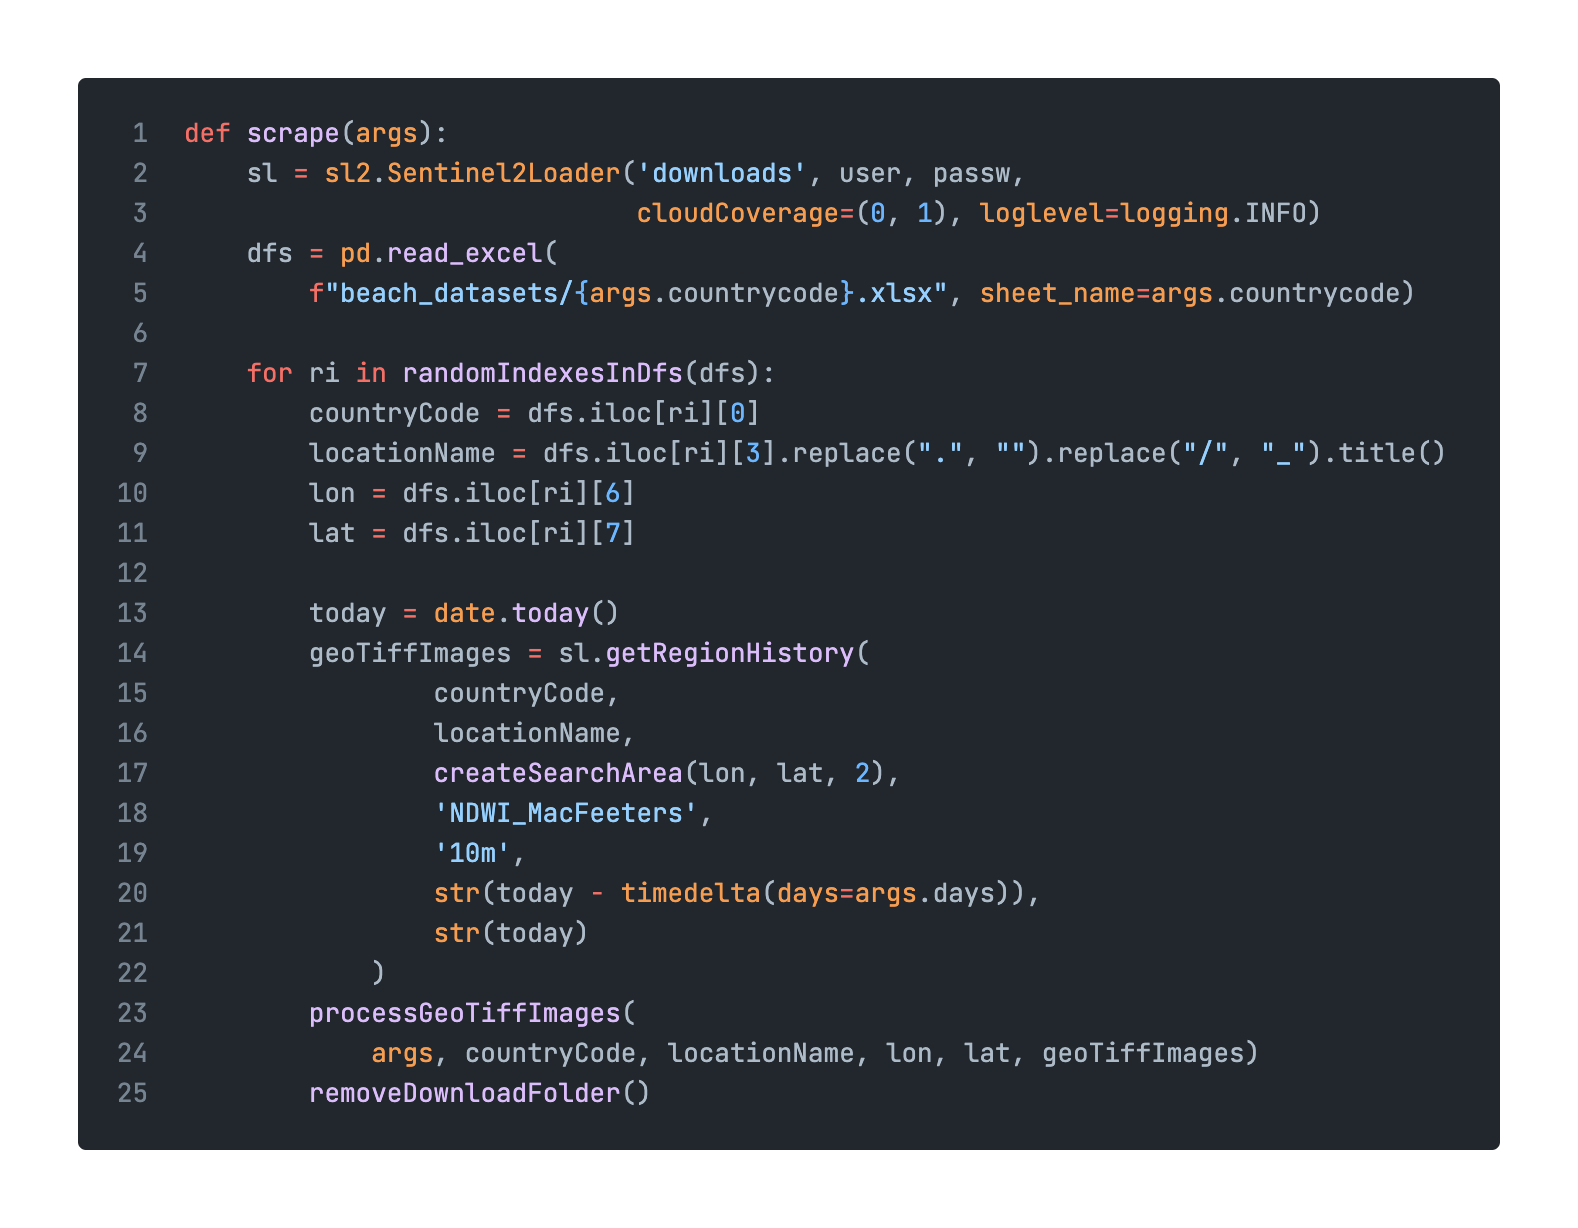
\includegraphics[width=\textwidth]{sentinel-satellite-scraper-scrape.png}
    \caption{The \emph{scrape(args)} methodh that is the entry point of the \acrshort{sss}.}
    \label{fig:sentinel-satellite-scraper-scrape}
\end{figure}

The scrape method first instantiates the \emph{Sentinel2Loader} from the \emph{sentinelloader} library with the folder to download products too, the Copernicus user, the desired cloud coverage percentage, and the log level. After this the locations to scrape for are read in from one of many excel files located in the scrapers directory. Each of these Excel files contains geolocations on beaches in a specific country. After this, the main scraping loop begins, where it randomly selects a non-processed beach and proceeds. This is a deliberate choice as the Copernicus API restricts the number of offline products that can be downloaded to 20 each day, and mixing up which locations we query historical data from ensures we use this retries on differently each time the script is run.
Next the different needed parameters are extracted from the excel data, and the process of downloading products, combining bands, and cropping the resulting images is started by the \emph{getRegionHistory(...)} method call. This call is called with the country code, the location name, a search area which is a geoshape that defines the boundary of the location of interest, the index we want to use to combine bands, the spatial resolution, the from date and lastly the to date.
As illustrated the combination of bands happens accordingly to the \acrfull{ndwi}. The \acrshort{ndwi} combines the bands into an image that differentiates water from land. The \acrshort{ndwi} uses a simple formula to combine band 3 and band 8 to give a value between 0 and 1 for each pixel that indicates the chance of that pixel being either water or land.

\[ NDWI = \dfrac{B3 - B8}{B3 + B8} \]

Furthermore, the cropping of the image relies on the provided geo polygon that defines the boundaries of the location of interest. It automatically crops out this location of interest from the downloaded product(s). In cases where the location of interest covers multiple products, the \emph{sentinelloader} library is able to download, combine and crop the image from various products, so no data is lost.

After having downloaded products, combined bands and cropped the resulting image, custom pre-processing is done on the resulting image, to color it based on the \acrshort{NDWI} values, and to ensure the image size is as compact as possible. This work happens in the \emph{processGeoTiffImages(...)}.

\begin{figure}[h!]
    \centering
    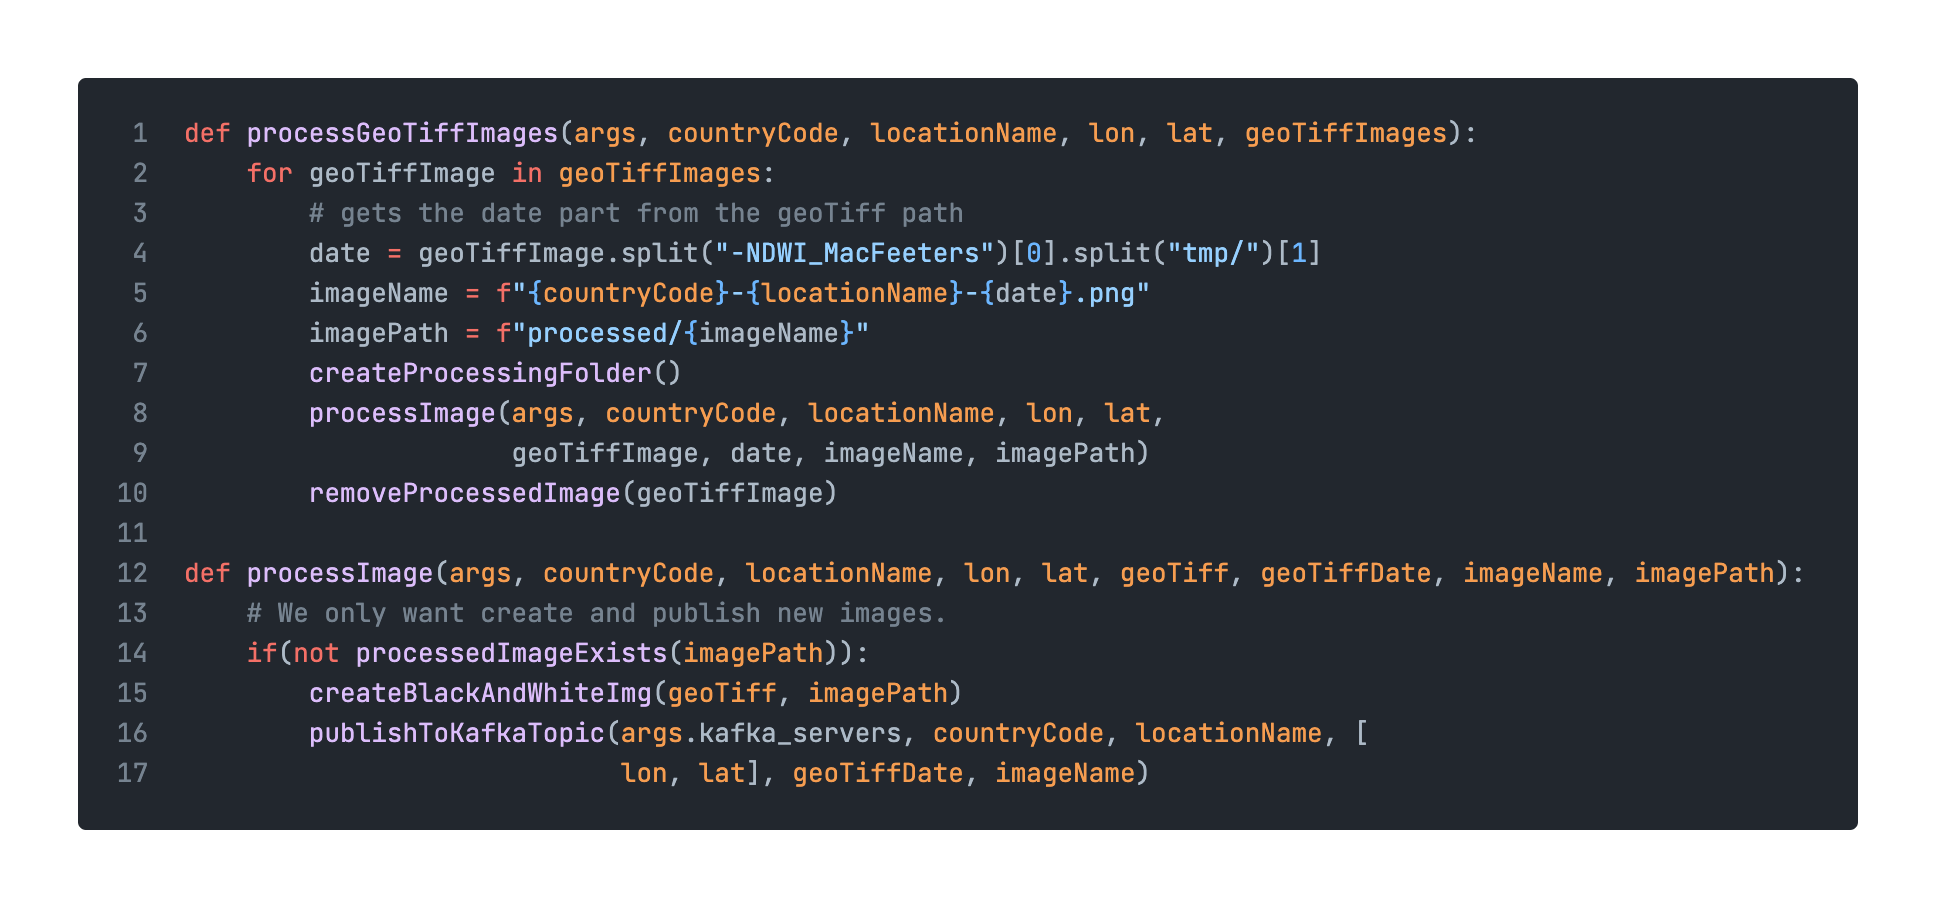
\includegraphics[width=\textwidth]{sentinel-satellite-scraper-pre-processing.png}
    \caption{The \emph{scrape(args)} methodh that is the entry point of the \acrshort{sss}.}
    \label{fig:sentinel-satellite-scraper-pre-processing}
\end{figure}

%https://sentinel.esa.int/documents/247904/685211/Sentinel-2-Products-Specification-Document

%https://gisgeography.com/sentinel-2-bands-combinations/

%https://en.wikipedia.org/wiki/Normalized_difference_water_index

This could be a data storage problem, but the \acrshort{sss} does not need to save these large products in order to pre-process them, and thus the products can safely be removed whenever they have been processed. Removal of processed images enable us to enjoy the extra detail that 10m imagery provides, and it is very useful to increase the precision of the results.

\subsection{NDWI Analyzer}\label{subsec:ndwi-analyzer}

– Purpose (Why?)
– Context (When?)
– Description (How?)

\subsection{WebAPI}

\subsection{EcoBeach App}






\chapter{Conclusion}

\section*{Future work}
- Future work

\printnoidxglossary[type=acronym]
\printbibliography[heading=bibintoc]

\appendix
\newgeometry{top=0cm}
\chapter{Infrastructure Diagram}\label{ch:infrastructure-diagram}
\begin{figure}[h!]
    \centering
    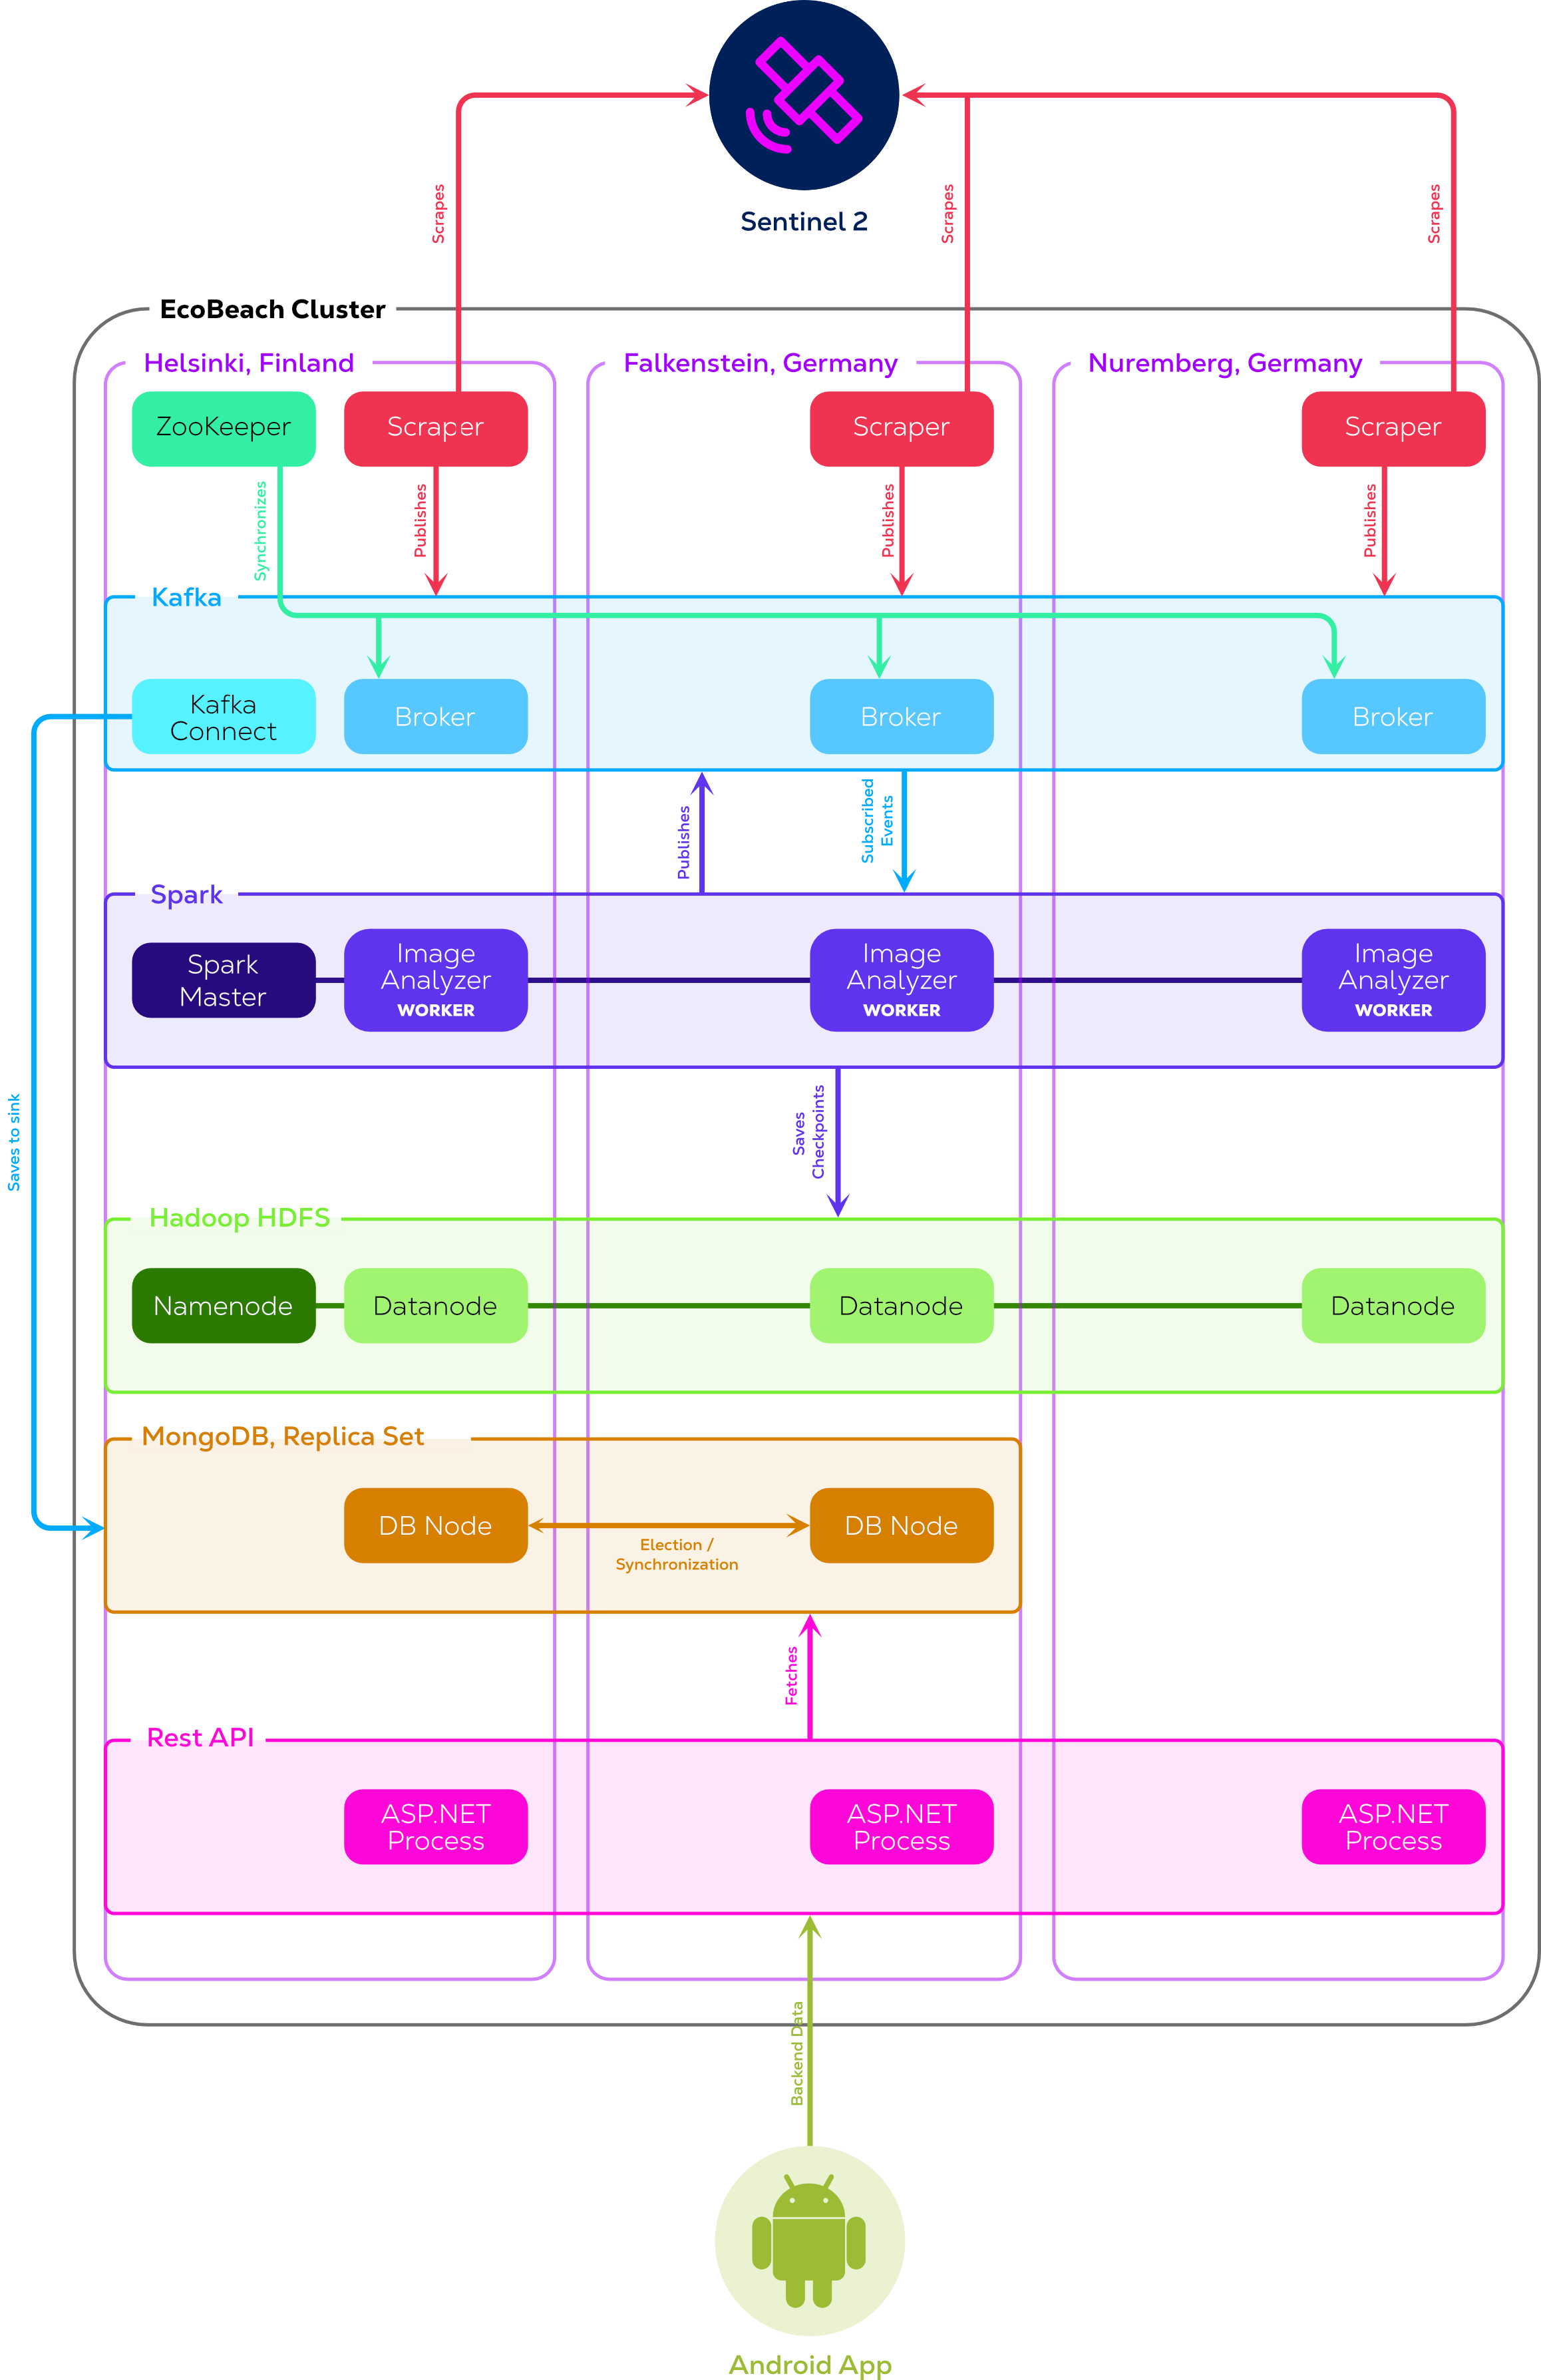
\includegraphics[width=0.735\textwidth]{small_infrastructure-2.png}
    \caption{The infrastructure of EcoBeach and how the included services relate to each other.}
\end{figure}
\restoregeometry
\end{document}